% ========================================
%	Header einbinden
% ========================================

\documentclass[bibtotoc,titlepage]{scrartcl}

% Deutsche Spracheinstellungen
\usepackage[ngerman,german]{babel, varioref}
\usepackage[T1]{fontenc}
\usepackage[utf8]{inputenc}

%\usepackage{marvosym}

\usepackage{amsfonts}
\usepackage{amssymb}
\usepackage{amsmath}
\usepackage{amscd}
\usepackage{amstext}

\usepackage{longtable}

%\usepackage{bibgerm}

\usepackage{footnpag}

\usepackage{ifthen}                 %%% package for conditionals in TeX
\usepackage[amssymb]{SIunits}
%Für textumflossene Bilder und Tablellen
%\usepackage{floatflt} - veraltet

%Für Testzwecke aktivieren, zeigt labels und refs im Text an.
%\usepackage{showkeys}

% Abstand zwischen zwei Absätzen nach DIN (1,5 Zeilen)
% \setlength{\parskip}{1.5ex plus0.5ex minus0.5ex}

% Einrückung am Anfang eines neuen Absatzes nach DIN (keine)
%\setlength{\parindent}{0pt}

% Ränder definieren
% \setlength{\oddsidemargin}{0.3cm}
% \setlength{\textwidth}{15.6cm}

% bessere Bildunterschriften
%\usepackage[center]{caption2}


% Problemlösungen beim Umgang mit Gleitumgebungen
\usepackage{float}

% Nummeriert bis zur Strukturstufe 3 (also <section>, <subsection> und <subsubsection>)
%\setcounter{secnumdepth}{3}

% Führt das Inhaltsverzeichnis bis zur Strukturstufe 3
%\setcounter{tocdepth}{3}
\usepackage[version=3]{mhchem}
	\mhchemoptions{minus-sidebearing-left=0.06em, minus-sidebearing-right=0.11em}
\usepackage{exscale}

\newenvironment{dsm} {\begin{displaymath}} {\end{displaymath}}
\newenvironment{vars} {\begin{center}\scriptsize} {\normalsize \end{center}}


\newcommand {\en} {\varepsilon_0}               % Epsilon-Null aus der Elektrodynamik
\newcommand {\lap} {\; \mathbf{\Delta}}         % Laplace-Operator
\newcommand {\R} { \mathbb{R} }                 % Menge der reellen Zahlen
\newcommand {\e} { \ \mathbf{e} }               % Eulersche Zahl
\renewcommand {\i} { \mathbf{i} }               % komplexe Zahl i
\newcommand {\N} { \mathbb{N} }                 % Menge der nat. Zahlen
\newcommand {\C} { \mathbb{C} }                 % Menge der kompl. Zahlen
\newcommand {\Z} { \mathbb{Z} }                 % Menge der kompl. Zahlen
\newcommand {\limi}[1]{\lim_{#1 \rightarrow \infty}} % Limes unendlich
\newcommand {\sumi}[1]{\sum_{#1=0}^\infty}
\newcommand {\rot} {\; \mathrm{rot} \,}         % Rotation
\newcommand {\grad} {\; \mathrm{grad} \,}       % Gradient
\newcommand {\dive} {\; \mathrm{div} \,}        % Divergenz
\newcommand {\dx} {\; \mathrm{d} }              % Differential d
\newcommand {\cotanh} {\; \mathrm{cotanh} \,}   %Cotangenshyperbolicus
\newcommand {\asinh} {\; \mathrm{areasinh} \,}  %Area-Sinus-Hyp.
\newcommand {\acosh} {\; \mathrm{areacosh} \,}  %Area-Cosinus-H.
\newcommand {\atanh} {\; \mathrm{areatanh} \,}  %Area Tangens-H.
\newcommand {\acoth} {\; \mathrm{areacoth} \,}  % Area-cotangens
\newcommand {\Sp} {\; \mathrm{Sp} \,}
\newcommand {\mbe} {\stackrel{\text{!}}{=}}     %Must Be Equal
\newcommand{\qed} { \hfill $\square$\\}
\renewcommand{\i} {\imath}
\def\captionsngerman{\def\figurename{\textbf{Abb.}}}

%%%%%%%%%%%%%%%%%%%%%%%%%%%%%%%%%%%%%%%%%%%%%%%%%%%%%%%%%%%%%%%%%%%%%%%%%%%%
% SWITCH FOR PDFLATEX or LATEX
%%%%%%%%%%%%%%%%%%%%%%%%%%%%%%%%%%%%%%%%%%%%%%%%%%%%%%%%%%%%%%%%%%%%%%%%%%%%
%%%
\ifx\pdfoutput\undefined %%%%%%%%%%%%%%%%%%%%%%%%%%%%%%%%%%%%%%%%% LATEX %%%
%%%
\usepackage[dvips]{graphicx}       %%% graphics for dvips
\DeclareGraphicsExtensions{.eps,.ps}   %%% standard extension for included graphics
\usepackage[ps2pdf]{thumbpdf}      %%% thumbnails for ps2pdf
\usepackage[ps2pdf,                %%% hyper-references for ps2pdf
bookmarks=true,%                   %%% generate bookmarks ...
bookmarksnumbered=true,%           %%% ... with numbers
hypertexnames=false,%              %%% needed for correct links to figures !!!
breaklinks=true,%                  %%% breaks lines, but links are very small
linkbordercolor={0 0 1},%          %%% blue frames around links
pdfborder={0 0 112.0}]{hyperref}%  %%% border-width of frames
%                                      will be multiplied with 0.009 by ps2pdf
%
\hypersetup{ pdfauthor   = {Hannes Franke; Julius Tilly},
pdftitle    = {V301 Innenwiderstand und Leistungsanpassung}, pdfsubject  = {Protokoll FP}, pdfkeywords = {V301, Innenwiderstand, Leistungsanpassung},
pdfcreator  = {LaTeX with hyperref package}, pdfproducer = {dvips
+ ps2pdf} }
%%%
\else %%%%%%%%%%%%%%%%%%%%%%%%%%%%%%%%%%%%%%%%%%%%%%%%%%%%%%%%%% PDFLATEX %%%
%%%
\usepackage[pdftex]{graphicx}      %%% graphics for pdfLaTeX
\DeclareGraphicsExtensions{.pdf}   %%% standard extension for included graphics
\usepackage[pdftex]{thumbpdf}      %%% thumbnails for pdflatex
\usepackage[pdftex,                %%% hyper-references for pdflatex
bookmarks=true,%                   %%% generate bookmarks ...
bookmarksnumbered=true,%           %%% ... with numbers
hypertexnames=false,%              %%% needed for correct links to figures !!!
breaklinks=true,%                  %%% break links if exceeding a single line
linkbordercolor={0 0 1},
linktocpage]{hyperref} %%% blue frames around links
%                                  %%% pdfborder={0 0 1} is the default
\hypersetup{
pdftitle    = {V301 Innenwiderstand und Leistungsanpassung}, 
pdfsubject  = {Protokoll AP}, 
pdfkeywords = {V301, Innenwiderstand, Leistungsanpassung},
pdfsubject  = {Protokoll AP},
pdfkeywords = {V301, Innenwiderstand, Leistungsanpassung}}
%                                  %%% pdfcreator, pdfproducer,
%                                      and CreationDate are automatically set
%                                      by pdflatex !!!
\pdfadjustspacing=1                %%% force LaTeX-like character spacing
\usepackage{epstopdf}
%
\fi %%%%%%%%%%%%%%%%%%%%%%%%%%%%%%%%%%%%%%%%%%%%%%%%%%% END OF CONDITION %%%
%%%%%%%%%%%%%%%%%%%%%%%%%%%%%%%%%%%%%%%%%%%%%%%%%%%%%%%%%%%%%%%%%%%%%%%%%%%%
% seitliche Tabellen und Abbildungen
%\usepackage{rotating}
\usepackage{ae}
\usepackage{
  array,
  booktabs,
  dcolumn
}
\makeatletter 
  \renewenvironment{figure}[1][] {% 
    \ifthenelse{\equal{#1}{}}{% 
      \@float{figure} 
    }{% 
      \@float{figure}[#1]% 
    }% 
    \centering 
  }{% 
    \end@float 
  } 
  \makeatother 


  \makeatletter 
  \renewenvironment{table}[1][] {% 
    \ifthenelse{\equal{#1}{}}{% 
      \@float{table} 
    }{% 
      \@float{table}[#1]% 
    }% 
    \centering 
  }{% 
    \end@float 
  } 
  \makeatother 
%\usepackage{listings}
%\lstloadlanguages{[Visual]Basic}
%\allowdisplaybreaks[1]
%\usepackage{hycap}
%\usepackage{fancyunits}


\usepackage{pgf,tikz}
\usetikzlibrary{arrows}
% ========================================
%	Angaben für das Titelblatt
% ========================================

\title{Versuch 408 - Geometrische Optik\\				% Titel des Versuchs 
\large TU Dortmund, Fakultät Physik\\ 
\normalsize Anfänger-Praktikum}

\author{Jan Adam\\			% Name Praktikumspartner A
{\small \href{jan.adam@tu-dortmund.de}{jan.adam@tu-dortmund.de}}	% Erzeugt interaktiven einen Link
\and						% um einen weiteren Author hinzuzfügen
Dimitrios Skodras\\					% Name Praktikumspartner B
{\small \href{dimitrios.skodras@tu-dortmund.de}{dimitrios.skodras@tu-dortmund.de}}		% Erzeugt interaktiven einen Link
}
\date{08.Januar 2013}				% Das Datum der Versuchsdurchführung

% ========================================
%	Das Dokument beginnt
% ========================================

\begin{document}

% ========================================
%	Titelblatt erzeugen
% ========================================

\maketitle					% Jetzt wird die Titelseite erzeugt
\thispagestyle{empty} 				% Weder Kopfzeile noch Fußzeile

% ========================================
%	Der Vorspann
% ========================================

%\newpage					% Wenn Verzeichnisse auf einer neuen Seite beginnen sollen
%\pagestyle{empty}				% Weder Kopf- noch Fußzeile für Verzeichnisse

\tableofcontents

%\newpage					% eine neue Seite
%\thispagestyle{empty}				% Weder Kopf- noch Fußzeile für Verzeichnisse
%\listoffigures					% Abbildungsverzeichnis

%\newpage					% eine neue Seite
%\thispagestyle{empty}				% Weder Kopf- noch Fußzeile für Verzeichnisse
%\listoftables					% Tabellenverzeichnis
\newpage					% eine neue Seite


% ========================================
%	Kapitel
% ========================================

\section{Einleitung}
\setcounter{page}{1}
Die geometrische Optik ist als Grenzfall der Wellenoptik ein Bereich der Physik, welcher sich des Strahlenmodells des Lichts bedient und
den Weg des Lichts auf ausschließlich geometrische Art und Weise formuliert. Neben der Verifizierung des Abbildungsgesetzes und der 
Linsengleichung, werden im Zuge des Experimentsdie Methoden von Bessel bzw. Abbe verwandt, um die Brennweite einer Sammellinse oder 
eines Linsensystems zu bestimmen.

\section{Theorie}
\subsection{Linsen - Arten und Eigenschaften}
Kernstück der geometrischen Optik sind die Linsen, welche grundsätzlich aus optisch dichterem Material als Luft bestehen. Nach dem 
Snelliusschem Brechungsgesetz wird Licht an der Grenzfläche solcher Materialien verschiedener optischer Dichte gebrochen. Wie das Licht
gebrochen wird, hängt vom Winkel des einfallenden Strahls ab. So unterscheidet man zwischen Sammellinsen und Streulinsen. 

\begin{figure}[H]
 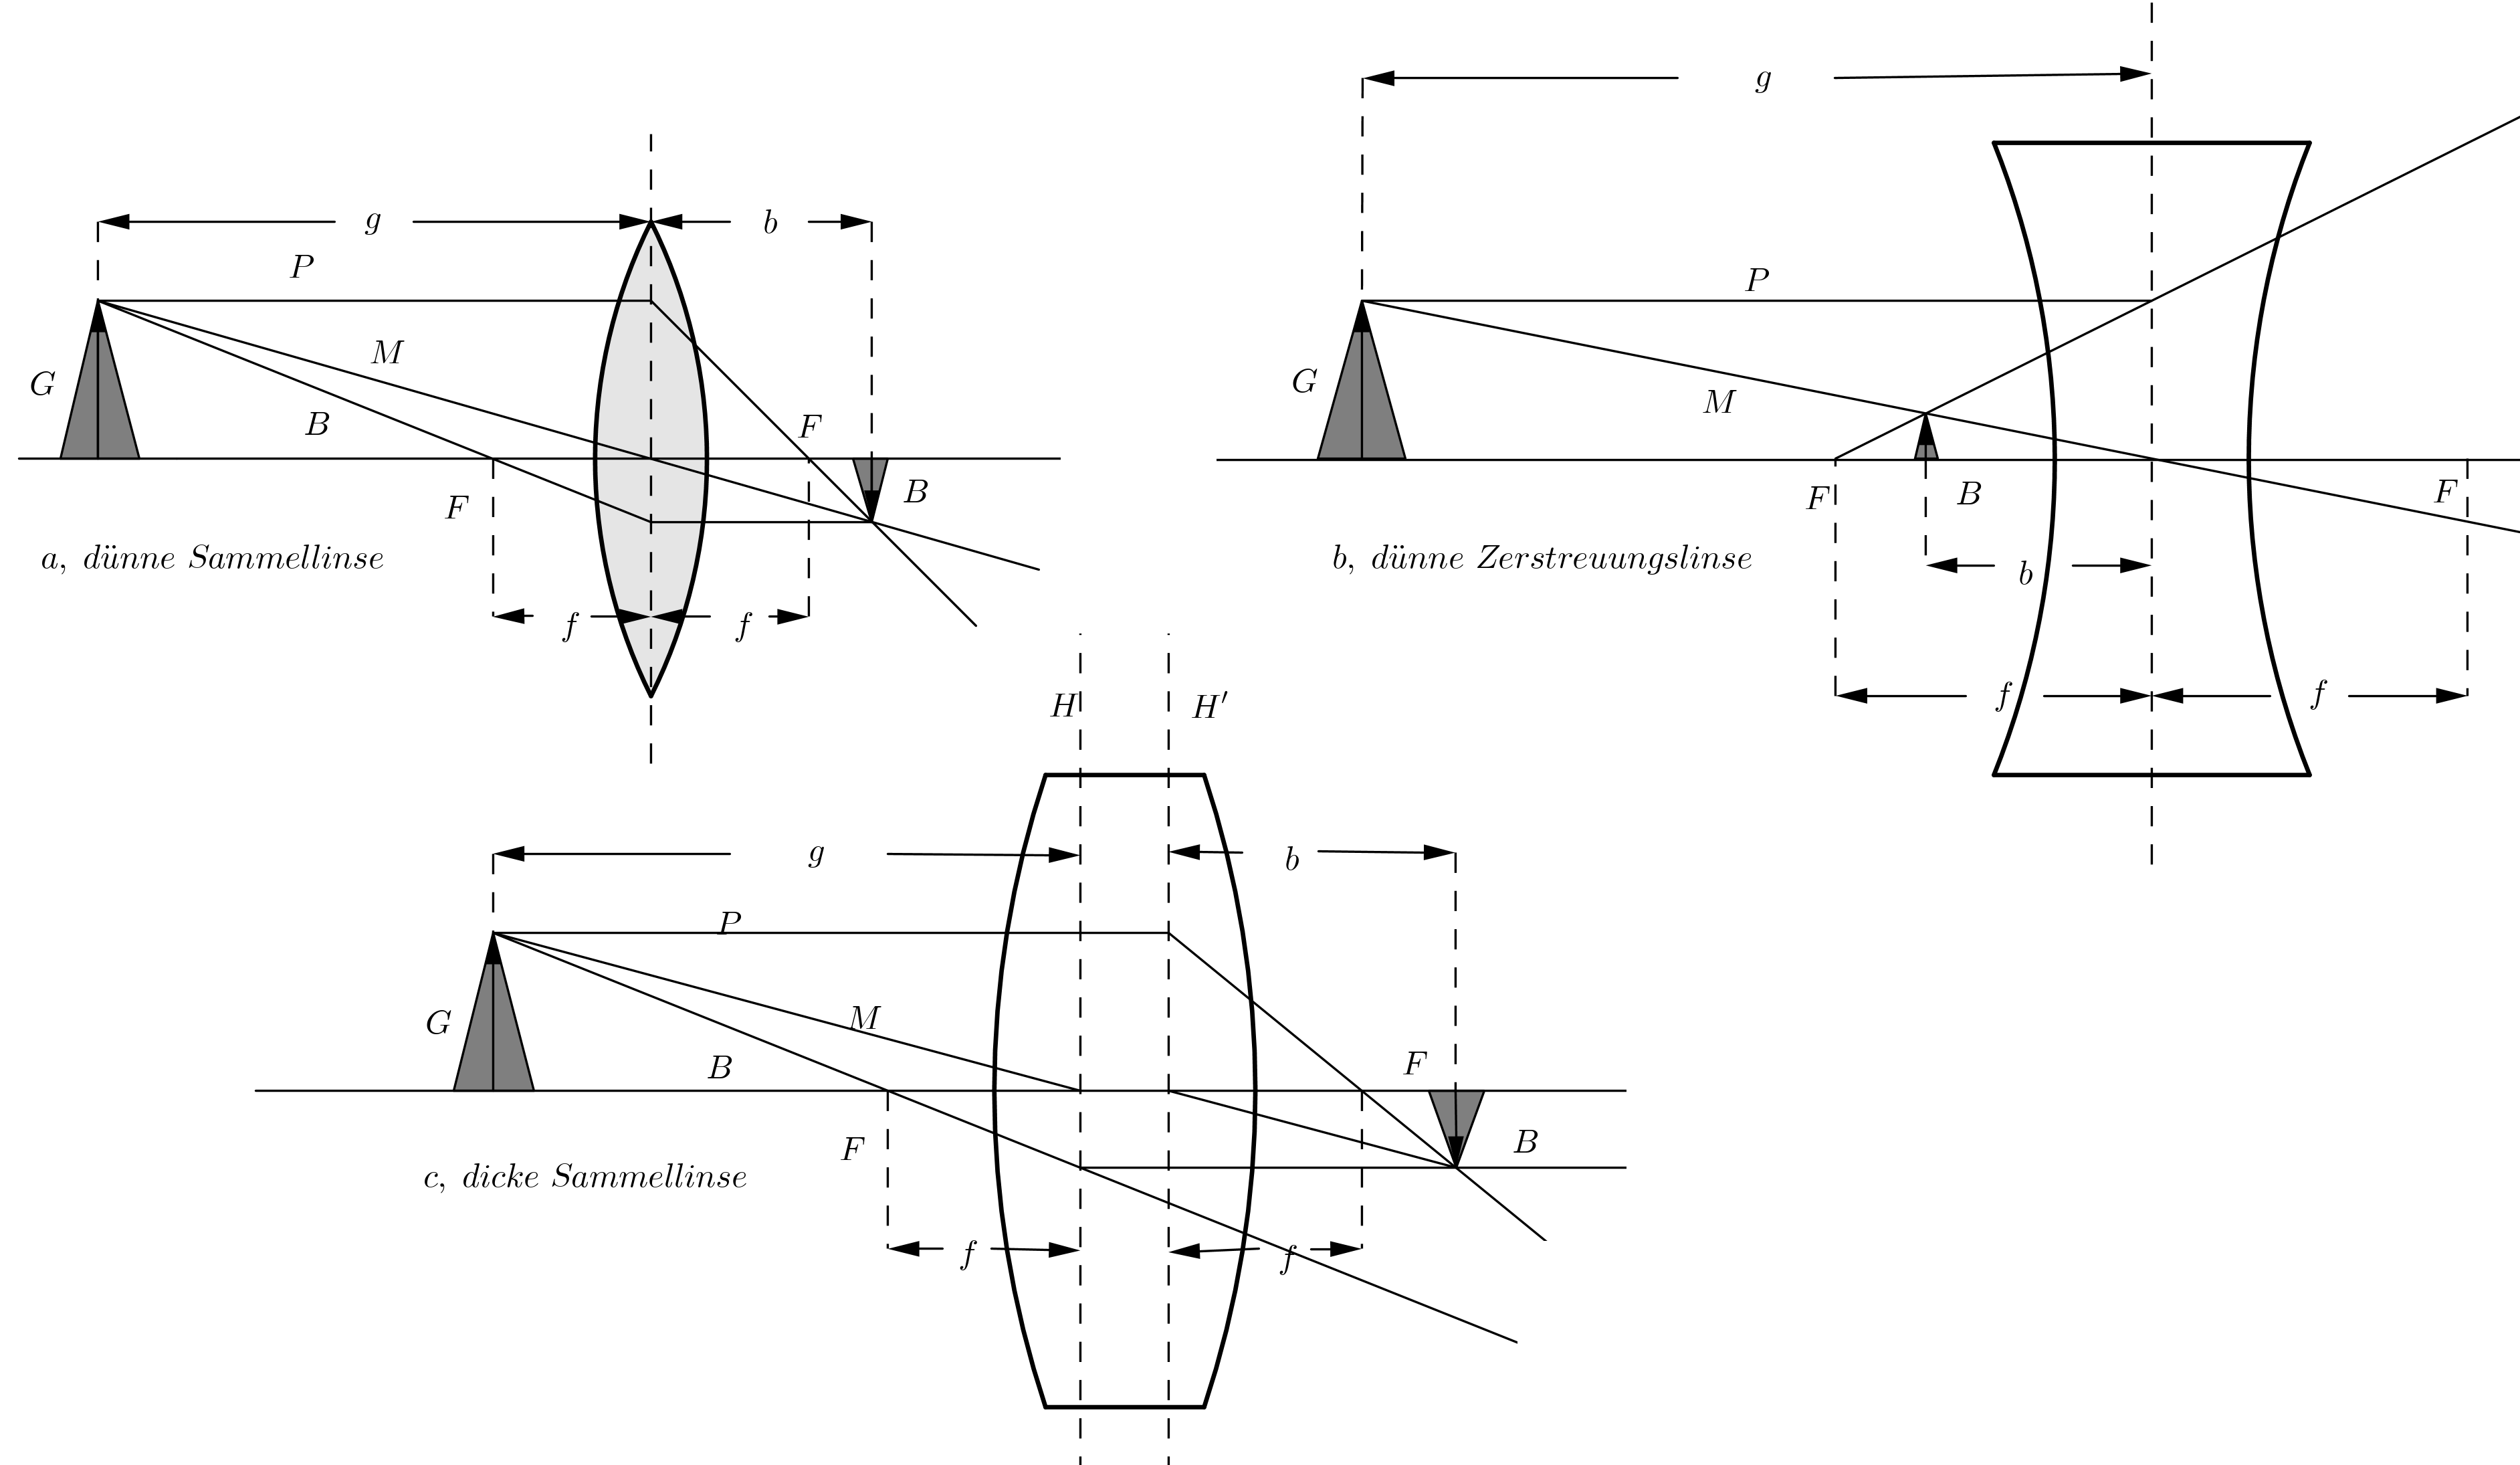
\includegraphics[width=\textwidth]{pics/408a.png}
 \centering
 \caption{Bildkonstruktionen: a, dünne Sammellinse - b, dünne Streulinse - c, dicke Sammellinse}
 \label{linsen}
\end{figure}

Charakterisiert sind Linsen durch ihre Brennweite $f$. sie ist die Distanz von der Mittelachse der Linse, in der paralleles Licht von
einer Sammellinse in einem Punkt, dem Brennpunkt, gebündelt wird. Wenn die Brennweite, sowie die Bildweite $b$ positiv sind, entsteht
ein reelles Bild (a,). Sind sie negativ, entsteht ein virtuelles Bild (b,). Die beiden Bildkonstruktionen in \ref{linsen} für dünne
Linsen sind durch die Reduktion der Brechung an der Mittelebene realisierbar. Hingegen bei dicken Linsen ist dies nicht durchführbar.
Daher werden die Hauptebenen H und H' hergenommen, an denen die Brechung geschieht. Zur Konstruktion werden der Parallelstrahl $P$, der
Mittelpunktstrahl $M$, sowie der Brennstrahl $B$ zu Hilfe genommen. Aus diesen Konstruktionen leitet sich das Abbildungsgesetz ab

\begin{formel}
 \begin{equation}
  V = \frac{B}{G} = \frac{b}{g}.
  \label{Abbildung}
 \end{equation}
 \caption*{\small{V = Abbildungsmaßstab, B = Bildhöhe, G = Gegenstandshöhe, g = Gegenstandsweite}}
\end{formel}

Hieraus ergibt sich für dünne Linsen die Linsengleichung zu

\begin{equation}
 \frac1f = \frac1b + \frac1g.
 \label{Linsengleichung}
\end{equation}

Bei dicken Linsen werden zur Erhaltung der Gültigkeit der Linsengleichung die Brennweite, die Gegenstandsweite, sowie die Bildweite 
zur jeweiligen Hauptebene bestimmt. 

\subsection{Abbildungsfehler - sphärisch und chromatisch}

\begin{wrapfigure}[20]{r}{0.5 \textwidth}
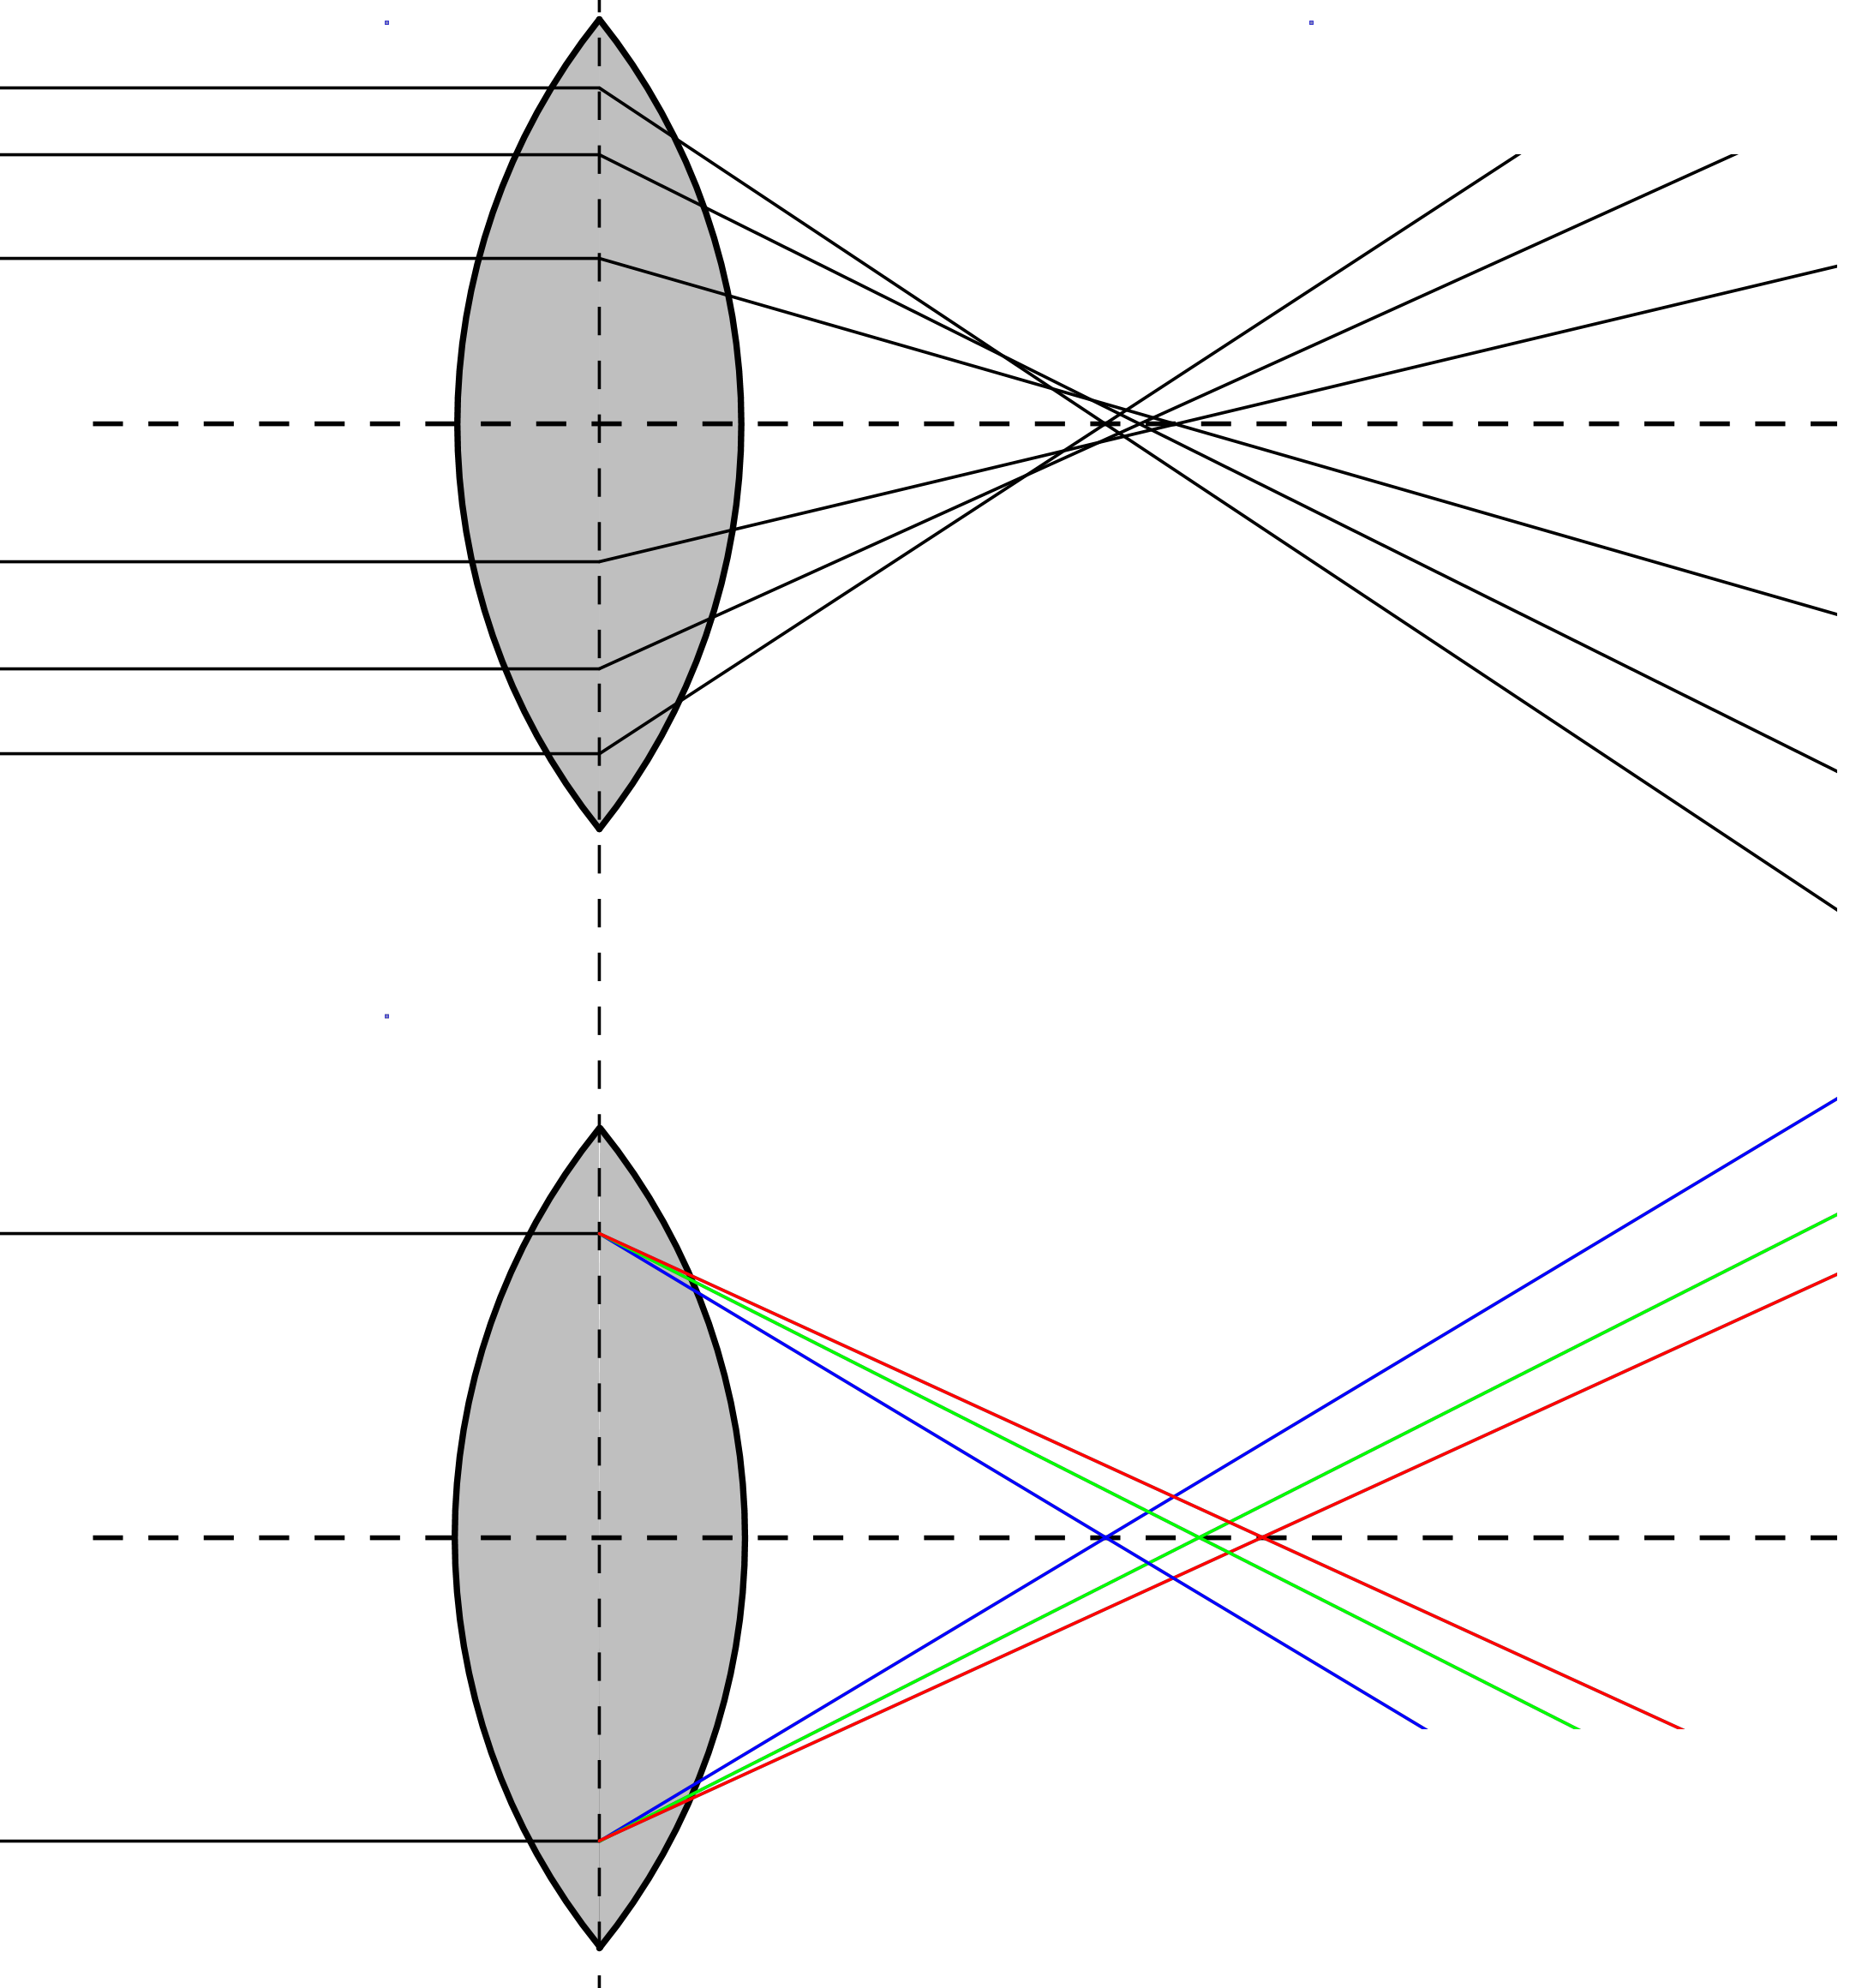
\includegraphics[width = 0.5 \textwidth]{pics/408b.png}  
\caption{sphärische (oben) und chromatische (unten) Aberration}
\end{wrapfigure}


Die Annäherung der Reduktion auf die Mittelebene bzw. die Hauptebenen ist für sich nur für achsennahe Strahlen zulässig. So kommt
es bei achsenfernen Strahlen zu Abbildungsfehlern, oder Aberrationen, was zur Folge hat, dass das Objekt nicht scharf abgebildet
werden kann. Bei sphärischen Aberrationen kommt es dazu, dass der Brennpunkt achsenferner Strahlen näher an der Linsenachse liegt,
als jener der achsennahen. Somit laufen sie nicht alle im selben Punkt zusammen. 

Chromatische Aberration ist ebenfalls ein Nichtzusammentreffen verschiedener Strahlen. Hierbei werden die verschiedenen Wellenlängen
$\lambda$ verschieden stark am Linsenmaterial gebrochen, was auf einen wellenlängeabhängigen Brechungsindex zurückzuführen ist. Diese
Erscheinung wird Dispersion genannt.

\section{Durchführung}
\subsection{Versuchsaufbau}
Das vorliegende Experiment benutzt die Gesetze der geometrischen Optik. Maßgeblich für Untersuchungen in diesem Bereich ist eine Lichtquelle,
ein abzubildendes Objekt (Perl L), sowie ein optisches Element, welches den Strahlengang beeinflusst und schließlich ein Schirm zur
Visualisierung. Die genannten Bauteile sind in Abbildung \ref{aufbau} dargestellt. Das optische Element und der Schirm sind auf der optischen
Bank mittels Reitern verschiebbar.

\begin{figure}[H]

\begin{tikzpicture}[line cap=round,line join=round,>=triangle 45,x=0.7cm,y=0.7cm]
\clip(-4.47,-4.72) rectangle (18.61,8.37);
\fill[fill=black,fill opacity=0.75] (-3,-3) -- (-2.5,-2) -- (-2,-3) -- cycle;
\fill[fill=black,fill opacity=0.75] (16,-3) -- (15.5,-2) -- (15,-3) -- cycle;
\fill[fill=black,fill opacity=0.75] (6.51,-3) -- (7,-2) -- (7.5,-3) -- cycle;
\fill[fill=black,fill opacity=0.75] (0.5,-3) -- (1,-2) -- (1.5,-3) -- cycle;
\fill[fill=black,fill opacity=0.25] (-4,-3) -- (-4,-4) -- (17,-4) -- (17,-3) -- cycle;
\draw (-4,-3)-- (17,-3);
\draw (-3,-3)-- (-2.5,-2);
\draw (-2.5,-2)-- (-2,-3);
\draw (-2,-3)-- (-3,-3);
\draw (16,-3)-- (15.5,-2);
\draw (15.5,-2)-- (15,-3);
\draw (15,-3)-- (16,-3);
\draw [line width=2pt] (-2.5,-2)-- (-2.5,1);
\draw [line width=2pt] (15.5,-2)-- (15.5,6);
\draw [line width=2pt] (-2.5,1)-- (-3,1);
\draw [line width=2pt] (-3,1)-- (-3,3);
\draw [line width=2pt] (-3,3)-- (-1,3);
\draw [line width=2pt] (-1,3)-- (-1,1);
\draw [line width=2pt] (-1,1)-- (-2.5,1);
\draw (6.51,-3)-- (7,-2);
\draw (7,-2)-- (7.5,-3);
\draw (7.5,-3)-- (6.51,-3);
\draw [line width=2pt] (7,-2)-- (7,0);
\draw [line width=2pt] (7,0)-- (7,4);
\draw [dash pattern=on 5pt off 5pt] (-1,2)-- (-0.5,2.28);
\draw [dash pattern=on 5pt off 5pt] (-1,2)-- (-0.35,2);
\draw [dash pattern=on 5pt off 5pt] (-1,2)-- (-0.49,1.63);
\draw (3.94,6.54) node[anchor=north west] {$ g $};
\draw (10.91,6.58) node[anchor=north west] {$b$};
\draw [->] (3,6) -- (1,6);
\draw [->] (5,6) -- (7,6);
\draw [->] (10,6) -- (7,6);
\draw [->] (12,6) -- (15.5,6);
\draw (0.5,-3)-- (1,-2);
\draw (1,-2)-- (1.5,-3);
\draw (1.5,-3)-- (0.5,-3);
\draw [line width=2pt] (1,-2)-- (1,0);
\draw [line width=2pt] (1,0)-- (1,4);
\draw (-4,-3)-- (-4,-4);
\draw (-4,-4)-- (17,-4);
\draw (17,-4)-- (17,-3);
\draw (5.06,5.19) node[anchor=north west] {$optisches \ Element$};
\draw (0.4,5.21) node[anchor=north west] {$Perl \ L$};
\draw (-4.39,5.17) node[anchor=north west] {$Halogenlampe$};
\draw (13.3,5.21) node[anchor=north west] {$Schirm$};
\draw [line width=2pt] (0,0)-- (2,0);
\draw [line width=2pt] (6,0)-- (8,0);
\draw (-4,-3)-- (-4,-4);
\draw (-4,-4)-- (17,-4);
\draw (17,-4)-- (17,-3);
\draw (17,-3)-- (-4,-3);
\end{tikzpicture}
\end{document}
\caption{Versuchsaufbau mit verschiebbarem optischem Element und Schirm}
\label{aufbau}
\end{figure}

\subsection[Messung von Gegenstandsweite und Bildweite]{Bestimmung der Brennweite durch Messung der Gegenstandsweite und Bildweite}
Im ersten Versuchsteil ist das optische Element eine Sammellinse bekannter Brennweite $f$. Nachdem die Gegenstandsweite $g$ eingestellt ist,
wird der Schirm entsprechend verschoben, sodass das entstehende Bild scharf ist. Die Distanz vom Schirm zur Linse ist die Bildweite $b$.
Die Linsengleichung \eqref{Linsengleichung} soll verifiziert werden. Die Messungen werden anschließend für eine Linse unbekannter Brennweite
wiederholt.

\begin{figure}
 \definecolor{qqqqff}{rgb}{0,0,1}
\definecolor{qqffqq}{rgb}{0,1,0}
\definecolor{ffqqqq}{rgb}{1,0,0}
\begin{tikzpicture}[line cap=round,line join=round,>=triangle 45,x=0.5cm,y=0.5cm]
\clip(-3.02,-4.71) rectangle (16.1,6.28);
\draw [->,line width=1.6pt] (0,-4.4) -- (0,6);
\draw [->,line width=1.6pt] (-0.4,-4) -- (12,-4);
\draw [dash pattern=on 4pt off 4pt] (0,0)-- (4,0);
\draw [dash pattern=on 4pt off 4pt] (4,0)-- (4,-4);
\draw [color=ffqqqq] (0,4)-- (8,-4);
\draw [color=qqffqq] (0,3)-- (9.33,-4);
\draw [color=qqqqff] (0,5)-- (7.22,-4);
\draw (4.48,0.78) node[anchor=north west] {$A$};
\draw (7.06,-4.02) node[anchor=north west] {$g_1$};
\draw (8.06,-4.02) node[anchor=north west] {$g_2$};
\draw (9.24,-4.02) node[anchor=north west] {$g_3$};
\draw (-0.99,5.47) node[anchor=north west] {$b_1$};
\draw (-1.02,4.45) node[anchor=north west] {$b_2$};
\draw (-1.04,3.48) node[anchor=north west] {$b_3 $};
\draw (1.78,-0.09) node[anchor=north west] {$f$};
\end{tikzpicture}

 \caption{Die Präzision der Geraden durch A ist ein Maß für die Messgenauigkeit.}
\end{figure}

\subsection[Methode von Bessel]{Bestimmung der Brennweite einer Linse nach der Methode von Bessel}
Bei der Methode von Bessel handelt es sich um ein Verfahren der Brennweitenermittlung mittels Fixierung des Gegenstand-Schirm-Abstandes.
Innerhalb dieser Strecke werden zwei Linsenpositionen gesucht, bei denen das Bild scharf abgebildet wird. Es handelt sich bei den beiden
Positionen um eine symmetrische Anordnung, sodass folgende Relation gilt

\begin{equation}
 b_1 = g_2, \qquad \text{sowie} \qquad b_2 = g_1.
\end{equation}

\begin{figure}[H]
 \definecolor{qqffqq}{rgb}{0,1,0}
\definecolor{ffqqqq}{rgb}{1,0,0}
\definecolor{qqqqff}{rgb}{0,0,1}
\begin{tikzpicture}[line cap=round,line join=round,>=triangle 45,x=0.47cm,y=0.35cm]
\clip(-5.93,-9.97) rectangle (30.64,10.86);
\draw [line width=2pt,color=qqqqff] (-2,0)-- (-2,2);
\draw [shift={(-8,0)},fill=black,fill opacity=0.25]  plot[domain=-0.54:0.54,variable=\t]({1*11.66*cos(\t r)+0*11.66*sin(\t r)},{0*11.66*cos(\t r)+1*11.66*sin(\t r)});
\draw [shift={(12,0)},fill=black,fill opacity=0.25]  plot[domain=-0.54:0.54,variable=\t]({-1*11.66*cos(\t r)+0*11.66*sin(\t r)},{0*11.66*cos(\t r)+-1*11.66*sin(\t r)});
\draw [shift={(24,0)},dash pattern=on 8pt off 8pt,fill=black,fill opacity=0.1]  plot[domain=2.6:3.68,variable=\t]({1*11.66*cos(\t r)+0*11.66*sin(\t r)},{0*11.66*cos(\t r)+1*11.66*sin(\t r)});
\draw [shift={(4,0)},dash pattern=on 8pt off 8pt,fill=black,fill opacity=0.1]  plot[domain=2.6:3.68,variable=\t]({-1*11.66*cos(\t r)+0*11.66*sin(\t r)},{0*11.66*cos(\t r)+-1*11.66*sin(\t r)});
\draw [line width=1.2pt] (-2,2)-- (2,2);
\draw [dash pattern=on 8pt off 8pt] (-2,2)-- (14,2);
\draw [dash pattern=on 8pt off 8pt] (14,2)-- (18,-0.5);
\draw [dash pattern=on 8pt off 8pt] (-2,2)-- (18,-0.5);
\draw [line width=1.2pt] (-2,2)-- (18,-8);
\draw [line width=1.2pt] (2,2)-- (18,-8);
\draw [dash pattern=on 8pt off 8pt] (14,8)-- (14,-8);
\draw [dash pattern=on 8pt off 8pt] (2,-8)-- (2,8);
\draw [line width=1.6pt] (24,0)-- (-4,0);
\draw [line width=2.4pt,color=ffqqqq] (18,0)-- (18,-0.5);
\draw [color=qqffqq] (18,0)-- (18,-8);
\draw [->] (0,-8) -- (2,-8);
\draw [->] (0,-8) -- (-2,-8);
\draw [->] (12,-8) -- (2,-8);
\draw [->] (12,-8) -- (18,-8);
\draw [->] (6,8) -- (-2,8);
\draw [->] (6,8) -- (14,8);
\draw [->] (16,8) -- (14,8);
\draw [->] (16,8) -- (18,8);
\draw [->] (8,6) -- (2,6);
\draw [->] (8,6) -- (14,6);
\draw [->] (8,10) -- (-2,10);
\draw [->] (8,10) -- (18,10);
\draw (-3.14,1.85) node[anchor=north west] {$G$};
\draw (18.65,-0.8) node[anchor=north west] {$B_1$};
\draw (18.65,-3.85) node[anchor=north west] {$B_2$};
\draw (-0.4,5.53) node[anchor=north west] {$L_1$};
\draw (15.2,5.49) node[anchor=north west] {$L_2$};
\draw (8.08,6.0) node[anchor=north west] {$d$};
\draw (8.08,10.8) node[anchor=north west] {$e$};
\draw (5.76,8.08) node[anchor=north west] {$g_2$};
\draw (16,7.65) node[anchor=north west] {$b_2$};
\draw (-0.83,-8.05) node[anchor=north west] {$g_1 = b_2$};
\draw (15.2,-8.02) node[anchor=north west] {$b_1 = g_2$};
\end{tikzpicture}
 \caption{Zwei verschiedene Linsenstellungen mit je einem scharfen vergrößerten bzw. verkleinertem Abbild}
\end{figure}

Wie zuvor gesagt, werden die beiden Konfigurationen bei festem Gegenstand-Schirm-Abstand gesucht und für mehrere Distanzen wiederholt.
Zur Ermittlung der Brennweite werden die Hilfsgrößen $e = g_1 + b_1$ und $d = g_1 - b_1$ eingeführt und wie folgt benutzt

\begin{equation}
 f = \frac{e^2-d^2}{4 \, e}.
 \label{Bessel}
\end{equation}

Zusätzlich wird in diesem Versuchsteil die chromatische Abberation untersucht, indem ein Rot- bzw. Blaufilter zwischen Lampe und Objekt
gehalten wird und nur die entsprechende Farbe zur Bildkonstruktion beiträgt. 

\subsection[Methode von Abbe]{Bestimmung der Brennweite eines Linsensystems nach der Methode von Abbe}
Die Bestimmung der Brennweite eines Linsensystems wird nach der Methode von Abbe die Lage der Hauptebenen durch den Abbildungsmaßstab V
ermittelt. $g$ und $b$ werden zu den jeweiligen Hauptebenen gemessen. Die Lage der Hauptebenen H und H' ist nicht bekannt. Ein freiwählbarer,
im Linsensystem fixierter Punkt A wird verwandt, um die Gegenstandsweite $g'$ und die Bildweite $b'$ leicht abzulesen. Es gelten folgende
in Abbildung \ref{abbe} nachvollziebare Relationen:

\begin{equation}
 g' = g + h = f \cdot \left( 1+ \frac1V \right) + h
 \label{eqabbe1}
\end{equation}
\begin{equation}
 b' = b + h' = f \cdot \left(1 + V \right) + h'
 \label{eqabbe2}
\end{equation}

\begin{figure}[H]
\begin{tikzpicture}[line cap=round,line join=round,>=triangle 45,x=0.7cm,y=0.6cm]
\clip(-4.01,-6.56) rectangle (17.02,5.42);
\draw [line width=2pt] (-1,1)-- (-1,0);
\draw [shift={(-2,0)},line width=1.6pt,fill=black,fill opacity=0.25]  plot[domain=-0.42:0.42,variable=\t]({1*9.85*cos(\t r)+0*9.85*sin(\t r)},{0*9.85*cos(\t r)+1*9.85*sin(\t r)});
\draw [shift={(16,0)},line width=1.6pt,fill=black,fill opacity=0.25]  plot[domain=-0.42:0.42,variable=\t]({-1*9.85*cos(\t r)+0*9.85*sin(\t r)},{0*9.85*cos(\t r)+-1*9.85*sin(\t r)});
\draw [shift={(17,0)},line width=1.6pt]  plot[domain=2.79:3.49,variable=\t]({1*11.7*cos(\t r)+0*11.7*sin(\t r)},{0*11.7*cos(\t r)+1*11.7*sin(\t r)});
\draw [shift={(-7,0)},line width=1.6pt]  plot[domain=2.79:3.49,variable=\t]({-1*11.7*cos(\t r)+0*11.7*sin(\t r)},{0*11.7*cos(\t r)+-1*11.7*sin(\t r)});
\draw [line width=1.6pt] (4,4)-- (6,4);
\draw [line width=1.6pt] (4,-4)-- (6,-4);
\draw [line width=2pt] (13.05,0)-- (13.05,-0.83);
\draw [dash pattern=on 5pt off 5pt] (-1,1)-- (4.48,0);
\draw [dash pattern=on 5pt off 5pt] (8.5,0)-- (13.05,-0.83);
\draw [dash pattern=on 5pt off 5pt] (-1,1)-- (4.48,-0.83);
\draw [dash pattern=on 5pt off 5pt] (4.48,-0.83)-- (13.05,-0.83);
\draw (4.48,4.96)-- (4.48,-5.02);
\draw (8.5,-5.04)-- (8.5,5);
\draw [line width=1.6pt] (-2,0)-- (14,0);
\draw (5.53,1.13) node[anchor=north west] {$A$};
\draw (3.78,5.49) node[anchor=north west] {$H$};
\draw (7.87,5.51) node[anchor=north west] {$H'$};
\draw [->] (4.48,-3.46) -- (-1.04,-3.48);
\draw [->] (-1.04,-3.48) -- (4.48,-3.46);
\draw [->] (6,-5) -- (-1,-5);
\draw [->] (-1,-5) -- (6,-5);
\draw [->] (13,-5) -- (6,-5);
\draw [->] (6,-5) -- (13,-5);
\draw [->] (8.5,-3.5) -- (13,-3.5);
\draw [->] (13,-3.5) -- (8.5,-3.5);
\draw [->] (4.48,-3.46) -- (6,-3.46);
\draw [->] (6,-3.46) -- (4.48,-3.46);
\draw [->] (8.5,-3.5) -- (6,-3.46);
\draw [->] (6,-3.46) -- (8.5,-3.5);
\draw [->] (4.48,1.99) -- (2,2);
\draw [->] (2,2) -- (4.48,1.99);
\draw (3.24,2.98) node[anchor=north west] {$f$};
\draw (1.95,-2.47) node[anchor=north west] {$g$};
\draw (10.85,-2.49) node[anchor=north west] {$b$};
\draw (2.33,-4.87) node[anchor=north west] {$g'$};
\draw (10.07,-4.87) node[anchor=north west] {$b'$};
\draw (7.06,-3.94) node[anchor=north west] {$h'$};
\draw (5.06,-3.94) node[anchor=north west] {$h$};
\draw (-1.77,1) node[anchor=north west] {$G$};
\draw (13.19,0.00) node[anchor=north west] {$B$};
\begin{scriptsize}
\fill [color=black] (2,0) circle (1.5pt);
\fill [color=black] (11,0) circle (1.5pt);
\fill [color=black] (6,0) circle (2.5pt);
\end{scriptsize}
\end{tikzpicture}
\caption{Das Linsensystem mit einer Streulinse und einer Sammellinse}
\label{abbe}
\end{figure}


\section{Auswertung}
\subsection{Gültigkeit von Linsengleichung und Abbildungsmaßstab}
Zunächst soll die Gültigkeit von Gleichung\eqref{Abbildung} und Gleichung\eqref{Linsengleichung} verifiziert werden. Dazu werden die Messwerte für die Gegenstandshöhe G, die Bildhöhe B, die Gegenstandsweite g und die Bildweite b aus der folgenden Tabelle entnommen und in die ensprechende Formel eingesetzt.\\
$V_1$ und $V_2$ sind die nach Gleichung \eqref{Abbildung} errechneten Längenverhältnisse von B zu G bzw. b zu g. Die Werte für f sind wiederum die errechneten Brennweiten in mm nach Gleichung \eqref{Linsengleichung}

\begin{table}[htbp]
\begin{center}
\begin{tabular}{|c|c|c|c !{\vrule width 1.5pt} c|c|c|}
G & g & b & B & $V_1$ & $V_2$ & f\\
\hline
3.0 & 11.7 & 65.1 & 16.3 & 5.43 & 5.59 & 98.82 \\ \hline
3.0 & 13.0 & 40.9 & 9.0 & 3.00 & 3.14 & 98.63 \\ \hline
3.0 & 14.0 & 33.8 & 7.0 & 2.33 & 2.41 & 99.00 \\ \hline
3.0 & 15.0 & 28.9 & 5.5 & 1.83 & 1.92 & 98.69 \\ \hline
3.0 & 16.0 & 25.3 & 4.6 & 1.53 & 1.58 & 98.01 \\ \hline
3.0 & 17.0 & 23.3 & 3.9 & 1.30 & 1.37 & 98.29 \\ \hline
3.0 & 18.0 & 21.6 & 3.3 & 1.10 & 1.20 & 98.08 \\ \hline
3.0 & 19.0 & 20.1 & 3.1 & 1.02 & 1.06 & 97.67 \\ \hline
3.0 & 20.0 & 19.0 & 2.9 & 0.97 & 0.95 & 97.44 \\ \hline
3.0 & 21.0 & 18.2 & 2.6 & 0.87 & 0.86 & 97.36 \\ \hline
\end{tabular}
\end{center}
\caption{Messwerte für Linse mit Brennweite f=100 mm}
\label{}
\end{table}

Anschließende Ausgleichs- und Fehlerrechnung ergeben schließlich als Brennweite der Linse:
\begin{align*}
97,7 \text{ mm}	\pm 0,45 \text{ mm}
\end{align*} Dies entspricht einer Abweichung von 2,34\% von den Herstellerangaben.

Die beiden Abbildungsverhältnisse $V_1$ und $V_2$ haben im Mittel eine Abweichung von 3,8\% zueinander.

\begin{table}[htbp]
\begin{center}
\begin{tabular}{|c|c!{\vrule width 1.5pt}c|}
g & b & f \\
\hline
10,0 & 41,0 & 267,71 \\ \hline
10,5 & 34,6 & 263,11 \\ \hline
11,0 & 29,8 & 259,64 \\ \hline
11,5 & 26,7 & 258,00 \\ \hline
12,0 & 25,2 & 258,46 \\ \hline
12,5 & 22,7 & 257,29 \\ \hline
13,0 & 21,7 & 258,24 \\ \hline
13,5 & 20,1 & 258,32 \\ \hline
14,0 & 19,0 & 259,07 \\ \hline
15,0 & 18,2 & 262,76 \\ \hline
\end{tabular}
\end{center}
\caption{Messwerte für Linse unbekannter Brennweite}
\label{}
\end{table}

Für die unbekannte Linse ergibt sich nach Auswertung der Messwerte eine Brennweite von
\begin{align*}
259,0 \text{ mm}	\pm2,09 \text{ mm}
\end{align*}

\subsection{Brechnungsindex nach Bessel und chromatische Abberation}
Nach Bessel lässt sich die Brennweite einer Linse ebenfalls nach Gleichung \eqref{Bessel} berechnen. Untersucht wird zudem, in wie weit Licht verschiedener Wellenlängen unterschiedlich stark gebrochen wird.\\
In Tabelle 2 stehen die gemessenen Werte für den Abstand d zwischen den beiden Linsenpositionen, für den Abstand e zwischen Gegenstand und Schirm, sowie die jeweiligen errechneten Brennweiten bei der Bestrahlung mit blauem (Tabelle 3) bzw. rotem (Tabelle 4) Licht:

\begin{table}[htbp]
\begin{center}
\begin{tabular}{|c|c|c|}
e & d & f \\
\hline
40,0 & 6,5 & 97,36 \\ \hline
45,0 & 16,1 & 98,19 \\ \hline
50,0 & 23,1 & 98,43 \\ \hline
55,0 & 29,6 & 97,67 \\ \hline
60,0 & 35,4 & 97,93 \\ \hline
65,0 & 41,2 & 97,37 \\ \hline
70,0 & 46,6 & 97,44 \\ \hline
75,0 & 51,8 & 98,23 \\ \hline
80,0 & 57,4 & 97,22 \\ \hline
85,0 & 62,6 & 97,24 \\ \hline
\end{tabular}
\end{center}
\caption{Messwerte aufgenommen nach der Methode von Bessel}
\label{tabbessel}
\end{table}

Die Werte für die Brennweite f errechnen sich nach Bessel mittels Gleichung \eqref{Bessel} 
Mittels Ausgleichs- und Fehlerrechnung folgt dann für die Brennweite:
\begin{align*}
 f= 97,7 \text{ mm}	\pm 0,45 \text{ mm}
\end{align*}

\begin{table}[htbp]
\begin{center}
\begin{tabular}{|c|c!{\vrule width 1.5pt}c|}
e & d & f\\
\hline
45,0 & 16,5 & 97,47 \\ \hline
50,0 & 23,4 & 97,62 \\ \hline
55,0 & 29,7 & 97,41 \\ \hline
60,0 & 35,3 & 98,23 \\ \hline
65,0 & 41,1 & 97,69 \\ \hline
\end{tabular}
\end{center}
\caption{Werte für blaues Licht (100 mm Brennweite)}
\label{tabblau}
\end{table}

Für blaues Licht zeigt die Linse ein Brechungsverhalten wie bei einer Linse mit einer Brennweite von:
\begin{align*}
97,7 \text{ mm}	\pm 0,323 \text{ mm}
\end{align*}

\begin{table}[htbp]
\begin{center}
\begin{tabular}{|c|c!{\vrule width 1.5pt}c|}
e & d & f\\
\hline
45,0 & 15,8 & 98,63 \\ \hline
50,0 & 23,2 & 98,20 \\ \hline
55,0 & 29,5 & 98,08 \\ \hline
60,0 & 35,3 & 98,23 \\ \hline
65,0 & 40,8 & 98,48 \\ \hline
\end{tabular}
\end{center}
\caption{Werte für rotes Licht (100 mm Brennweite)}
\label{tabrot}
\end{table}

Für rotes Licht zeigt die Linse ein Brechungsverhalten wie bei einer Linse mit einer Brennweite von:

\begin{align*}
98,3 \text{ mm}	\pm 0,22 \text{ mm}
\end{align*}


\subsection{Brechungsindex nach Abbe}

Nach Abbe lässt sich die Brennweite eines Linsensystems mittels Gleichungen \eqref{eqabbe1} bzw. \eqref{eqabbe2}. Hierfür wird b' bzw g' linear gegen $(1+V)$ bzw. $\left(1+\frac{1}{V}\right)$ aufgetragen und die Brennweite f als Steigung der Geraden abgelesen.

\begin{table}[htbp]
\begin{center}
\begin{tabular}{|c|c|c|c|}
G & g' & b' & B\\
\hline
3,0 & 10,0 & 70,3 & 5,0 \\ \hline
3,0 & 25,0 & 50,8 & 3,3 \\ \hline
3,0 & 30,0 & 44,8 & 2,5 \\ \hline
3,0 & 35,0 & 43,2 & 2,1 \\ \hline
3,0 & 40,0 & 39,5 & 1,7 \\ \hline
3,0 & 45,0 & 39,0 & 1,6 \\ \hline
3,0 & 50,0 & 37,1 & 1,3 \\ \hline
3,0 & 55,0 & 36,3 & 1,1 \\ \hline
3,0 & 60,0 & 35,9 & 1,1 \\ \hline
3,0 & 65,0 & 35,0 & 1,0 \\ \hline
\end{tabular}
\end{center}
\caption{Gemessene Abstände nach der Methode von Abbe - der erste Wert fließt wegen zu starker Abweichung nicht in die weitere Auswertung mit ein}
\label{}
\end{table}

\begin{figure}[H]
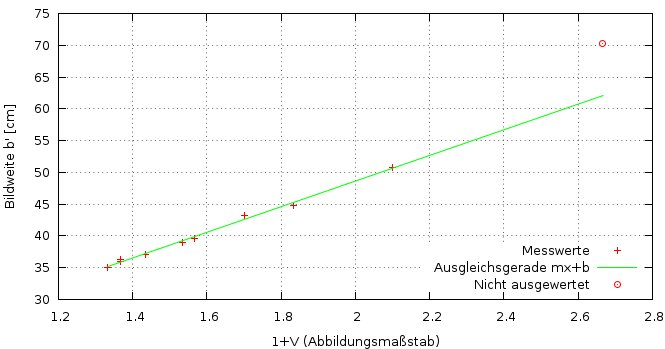
\includegraphics[width=0.8\textwidth]{pics/abbe1.jpg}
\caption{b' aufgetragen - errechnete Regressionsgrade}
\end{figure}

\begin{figure}[H]
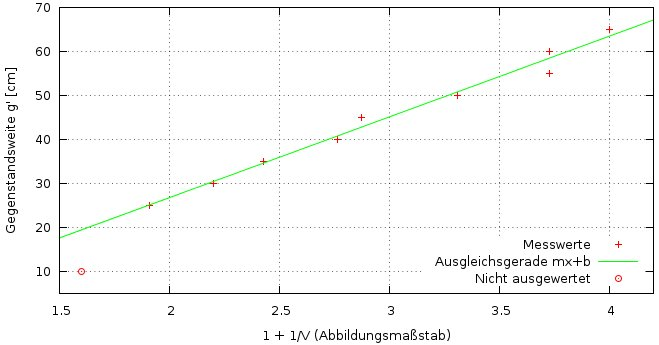
\includegraphics[width=0.8\textwidth]{pics/abbe2.jpg}
\caption{g' aufgetragen - errechnete Regressionsgrade}
\end{figure}


\begin{align*}
b': f&=20,2 \text{ mm}         \pm 0,54 \text{ mm}\\
g': f&=18,4 \text{ mm}          \pm 0,87 \text{ mm}
\end{align*}

\section{Diskussion}
Insgesamt stimmen alle Werte sehr gut mit den Erwartungen überein. Eine Abweichung der berechneten Brennweite von etwa 2\% zu den Herstellerangaben lässt auf einen systematischen Fehler beim Messen schließen. Da es nicht ganz eindeutig ist, wann die Abbildung wirklich scharf abgebildet wird, wurde vermutlich eine falsche Einstellung als "scharf" empfunden. Dass alle Werte gleichermaßen zu klein sind, bekräftigt diese Vermutung.\\
Gleiches gilt für den Abbildungsmaßstab V. Dass $V_1 = \frac{B}{G}$ und $V_2 = \frac{b}{g}$ eine Abweichung von etwa 3\% zueinander haben lässt sich vermutlich ebenfalls darauf zurückführen, dass das Bild bei der Messung nicht völlig scharf eingestellt war.\\
Für die chromatische Abberation ergibt sich, dass blaues Licht offenbar stärker im Glas gebrochen wird als rotes. Entsprechend liegt der Brennpunkt der Linse für blaues Licht dichter am Glas als für rotes Licht. Die Abweichung beträgt hier wieder nur etwa 2\%, für optische Geräte wie hochauflösende Kameras, kann dies aber durchaus problematisch sein.\\
Bei der Auswertung mit der Methode nach Abbe ergibt sich wie auch schon bei den vorherigen Rechnungen eine Abweichung zwischen beiden Messreihen. Wie schon zuvor liegt dies vermutlich daran, dass das Bild nicht vollständig scharf gestellt wurde, als die Werte aufgenommen worden sind. Dennoch sind die Zahlen durchaus plausibel und weichen auch nicht zu stark voneinander ab, so dass man von einer korrekten Auswertung ausgehen kann.

% ========================================
%	Literaturverzeichnis
% ========================================

%\bibliographystyle{plainnat}			% Bibliographie-Style auswählen
%\bibliography{BIBDATEI}			% Literaturverzeichnis

% ========================================
%	Das Dokument endent
% ========================================

\end{document}
